\section{Proposed Solution}
\label{sec:proposed_solution}

This project tries to fix the aforementioned problem by
introducing a proxy between the entity requesting the function execution and the
serverless function. This proxy will analyze each function's past history, by
looking at the time taken in past requests and make the decision of which runtime
environment \footnote{Runtime environment is the system where the serverless function will be executed, i.e., local network or one of the servers available in the cloud} should the request be forwarded to, see Figure
\ref{fig:request_func_high_level_diagram}. The proxy should be able to decide
between the local network of devices and one of the many available servers.

\begin{figure}[ht]
  \centering
  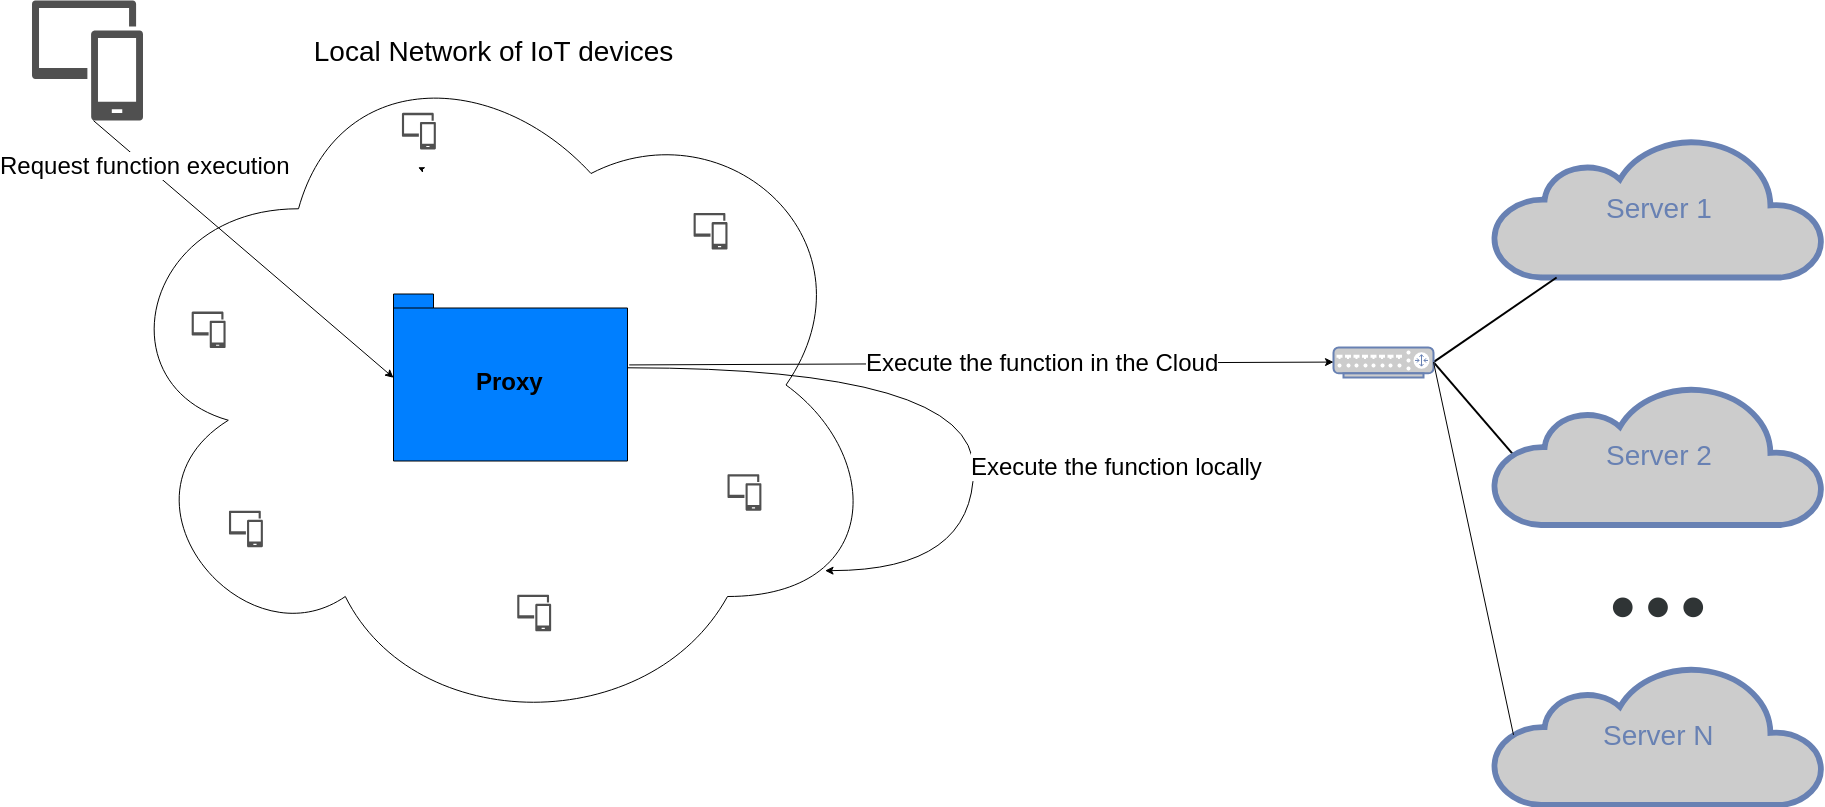
\includegraphics[width=0.5\textwidth]{diss-high-level-diagram.png}
  \caption{High level overview of project's architecture.}
  \label{fig:request_func_high_level_diagram}
\end{figure}

In order to improve fault-tolerance, in case of no Internet connection or if
one of the servers is not available if the request to the server fails, the proxy
should fallback to the local network. This way, even if the request to execute the function is forwarded to the server and fails, the function will still be executed locally.

The proxy is situated inside the local network of IoT devices and will forward the
request for a specific function to a gateway which forwards the function execution to
one of the IoT devices capable of executing the function. The load management,
containerization, replication, and clustering of the serverless functions is not
handled by the proxy, but it still has to be aware of the serverless functions
installed in the local network or any of the other runtime environments.

\subsection{Expected results and flow: Use cases}
\label{overview:usecases}
The following examples explain the expected results and decision-making of the
proposed solution. The decisions taken by the proxy are based only on previous
metrics of the time taken for the runtime environment to execute the function
(including network latency).

\subsubsection{Forward function execution to the cloud} \label{usecases:forward_cloud}

The use case in Figure \ref{fig:succ-cloud-deploy} exemplifies a situation where
the requested serverless function is hardware intensive, therefore taking a lot of
time to execute locally. Due to the high processing power of the cloud servers, it
is beneficial to forward the execution request to one of the cloud servers, even
when considering the connection latency. From the multiple available servers, it
will opt for the one that is physically nearest (lower latency).

\begin{figure}[ht]
  \begin{center}
    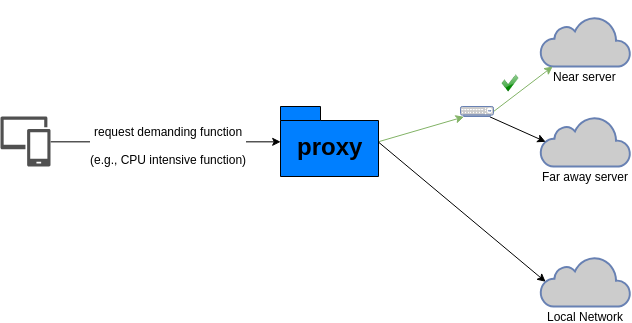
\includegraphics[width=0.5\textwidth]{diss-succ-cloud-deploy.png}
    \caption{Request for the execution of a demanding function to be executed. The proxy will forward the request to the cloud because due to the high processing  power of the cloud server, the function will be executed more quickly. The nearest server was chosen because of latency.}
    \label{fig:succ-cloud-deploy}
  \end{center}
\end{figure}

\subsubsection{Forward function execution to the local network}
\label{usecases:forward_local}

Contrary to the previous case, the Figure \ref{fig:succ-local-deploy} portrays a scenario where the requested serverless function is very light, being more beneficial to execute the function locally and avoid network latency. Despite the difference in power between the two environments, the previous metrics show that
the local environment is capable of satisfying the request more quickly.

\begin{figure}[ht]
  \begin{center}
    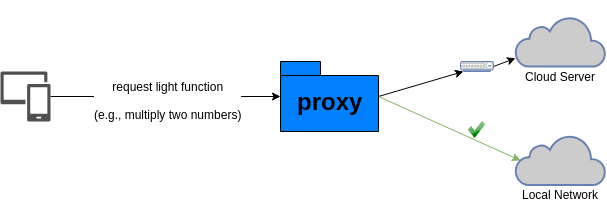
\includegraphics[width=0.5\textwidth]{diss-succ-local-deploy.png}
    \caption{Request for the execution of a simple, light function to be executed. The proxy will forward the request to be run locally, as there is no benefit in
    executing the function on the cloud.}
    \label{fig:succ-local-deploy}
  \end{center}
\end{figure}

\subsubsection{Fallback to the local network}
\label{usecases:fallback}

The Figure \ref{fig:fallback-local} depicts a scenario where the proxy first tries
to forward the request to one of the cloud servers (because it is more beneficial)
but fails in doing so. The proxy then decides to forward the request to the local
network, successfully completing the request. There are certain situations where
it is more favorable for the function to be executed on the cloud but it could
still be executed locally. Because it is not possible to always guarantee a
working connection, in these cases, if the connection fails the proxy will
fallback to execute function locally, assuring fail redundancy and the reliability
of the system.

\begin{figure}[ht]
  \begin{center}
    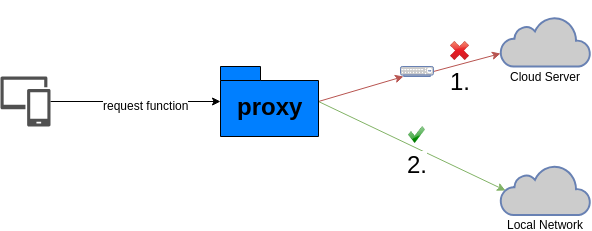
\includegraphics[width=0.5\textwidth]{diss-fallback-local.png}
    \caption{The request for the function execution to be in the cloud could not be satisfied (e.g., no internet connection). The proxy will then forward the
request for it to be executed in the local network.}
    \label{fig:fallback-local}
  \end{center}
\end{figure}

\subsubsection{Manual forward. Bypass the weighting process}
\label{usecases:manual_forward}

It should also be possible for the developer to bypass the weighting process (the
evaluation of the different runtime environments) and manually choose where to forward the
request. This option should be possible either in the setup process of the
function or as an argument of the request for the function execution. 

%\subsubsection*{Overall sequence} 
%In a very summarized way, the proxy when receiving a request will first decide, from
%a list of various runtime environments (the list must include the local network of
%devices and one or more cloud servers), where to forward the request to execute a
%serverless function. It will decide based on previous metrics of the time taken
%for the function to execute in the different runtime environments and will aim to
%choose the one with less time taken. It is also possible for the runtime
%environment to be manually configured in the request options or when setting up
%the proxy. If it decides to forward the request to the local network, it will
%just wait for it to execute. If it decides to execute the function in one of the
%cloud servers, it will make a request to the cloud server for it to execute the
%serverless function and if this request fails (e.g. because there is no connection to
%the server), it will then try to execute the function in the local network of
%devices. After having the response from the function execution, the proxy will
%answer with the response. A sequence diagram of this process summarized can be
%seen in \ref{fig:high_level_request_func_seq_diagram}.

%\begin{figure}[ht]
  %\begin{center}
    %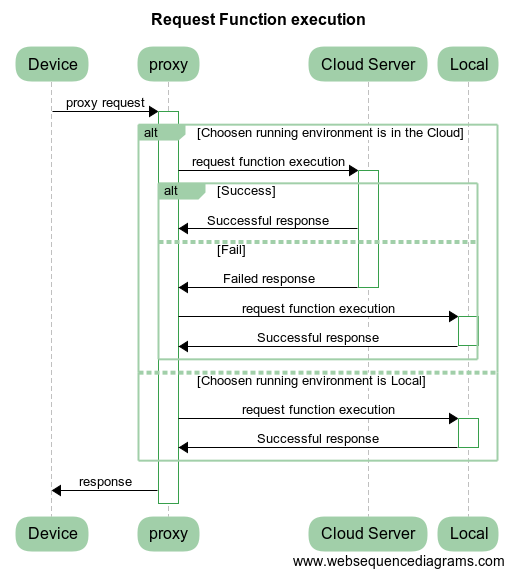
\includegraphics[width=0.5\textwidth]{diss-high-level-sequence-diagram.png}
    %\caption{High level sequence the whole process. This diagram sums the
        %decision-making of the project when trying to answer the request for the
        %function execution}
        %\label{fig:high_level_request_func_seq_diagram}
  %\end{center}
%\end{figure}

\subsection{Weighting the runtime environments}

In order to make the decision of which runtime environment to forward the function
to, there has to be some weighting process that will weight each of the runtime
environments and compare them. This process will gather information about the
different runtime environments and then make an accurate estimation of which one
is the best choice (less time took). This is similar to the Exploration vs
Exploitation problem presented in \ref{sec:sota_mab}. Therefore, the following
algorithms were implemented to handle the weighting process:

\begin{itemize}
    \item \textbf{Greedy} - Has no exploration, simply assigns the weight as the
        mean average time taken.
    \item \textbf{UCB1} - Uses Hoeffding's Inequality to balance between
        exploration and exploitation, but the cumulative regret will still be considerable.
    \item \textbf{Bayesian UCB} - Analyzes the reward distribution to make a very
        accurate prediction of the weight but requires previous knowledge about the environments.
\end{itemize}

The developer or device can choose which of the weighting algorithms will be used
for that request, in the options, but the default algorithm is UCB1. UCB1 was
selected as default because despite Bayesian UCB being better, it requires
previous knowledge about the environment, as stated in \ref{sota:bayesian_ucb}.

\subsection{Code components}

As it can be seen in Figure \ref{fig:component_diagram}, the proposed solution is
constituted of two main components, the \textbf{proxy} and the
\textbf{sample\_functions}. Each of these components is a package in itself.

\subsubsection{Packages}

\begin{itemize}
    \item \textbf{proxy} - The main package of the project responsible for
        all the logic. Deals with the reception of the request for the execution
        of a function, with the weighting of the environments in which the
        functions can run (locally or in the cloud in one of the multiple
        servers), and with the storage and retrieval of all metrics of previous
        function executions. 
    \item \textbf{sample\_functions} - The package that contains the serverless functions
        whose execution is going to be requested to the proxy package. This package is purely a sample with the purpose of simulating and analyzing resource demanding serverless functions (either light or heavy) and could be replaced by any other set of functions. The functions inside this package can be executed on either the local environment or on one of the servers (remote environments).
\end{itemize}

\subsubsection*{proxy}


All the different functions inside the proxy package communicate through HTTP and
expect to receive the content as application/json.

\begin{itemize}
    \item \textbf{proxy} - The main function through which all requests go through
        first. After receiving the list of weights associated with the execution of
        the requested function in each environment, it will choose the environment
        with the least weight and forward the execution of the serverless function
        to that runtime environment.
    \item \textbf{weight\_scale} - This function will analyze all the collected 
        metrics of the requested function and assign a weight to each runtime environment. It allows more than one algorithm for weight estimation.
    \item \textbf{get\_duration} - Retrieves the list of all the collected
        metrics of a function.
    \item \textbf{insert\_duration} - Store the time taken for a function to
        execute.
    \item \textbf{get\_overall\_stats} - Function that will return the summarized
        records of all the collected metrics for each function in each environment. Useful for analysis and evaluation of the results.
\end{itemize}

\begin{figure}[ht]
  \begin{center}
    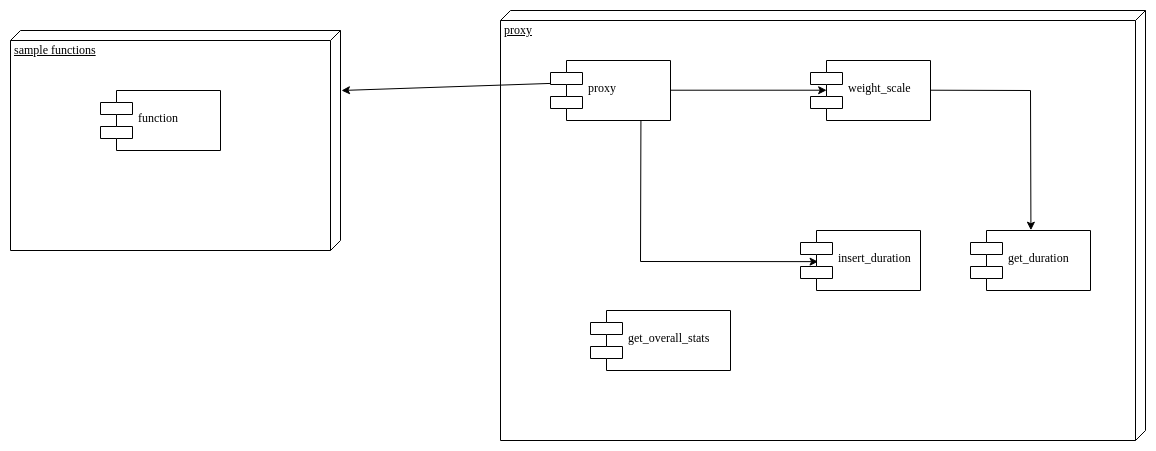
\includegraphics[width=0.5\textwidth]{diss-component-diagram}
    \caption{Component diagram of the project}
    \label{fig:component_diagram}
  \end{center}
\end{figure}

\subsubsection*{sample\_functions} \label{overview:sample_functions}

The serverless functions in this package have the purpose of simulating real serverless
functions for different purposes and execution times. The functions are aware of
the runtime environment they are being executed on and it is possible for them the answer
differently according to this. Here, the different time taken is simulated using a
\textit{wait} and using different values for different runtime environments.
 

\begin{itemize}
    \item \textbf{func\_light} - This function answers instantly, there should be
        no difference between executing the function locally or in the cloud,
        other than connection latency.
    \item \textbf{func\_heavy} - In this function there is a \textit{wait} of 2 seconds if
        it is executed locally or a \textit{wait} of 1 second if it is executed on the cloud. There should be no difference in the time taken across different cloud servers other than connection latency.
    \item \textbf{func\_super\_heavy} - similar to \textit{func\_heavy} but here the difference in time is bigger. There is a \textit{wait} of 4 seconds if the function is executed locally or a \textit{wait} of 2 seconds if the function is executed in the cloud.
    \item \textbf{func\_obese\_heavy} - This is a function that, due to its nature, it can
        only be executed in the cloud and its execution has been flagged as cloud-only. The proxy will not even try to run the function locally, it will always forward the request to the cloud. Because of this, there is no fallback to run locally.
\end{itemize}
